\section{多视角判别与残差重建探索}
\label{sec:ch06_multiview_residual_refiner}

多轮优化提高了当前判别器下的接受率，却未维持固定距离评价中的质量。本节从输出修正和判别信息两方面考察这一问题：条件残差修正器（Refiner）调整已有生成结果，全局（Global）、区域统计（Spatial）和时序（Temporal）分支分别检查不同响应特征。实验记录编号为P50，从$F_0$重新开始，而非续接上一节$F_3$，采用Seed 5001、单轮训练；两套VAE冻结，共享向量场与Refiner可训练。$F_{50}$表示本实验生成器的终点结果，$D_{50}$表示多视角判别器；下标50对应实验编号，不表示训练50轮。

Refiner逐帧拼接$\log(1+Y_0)$与$z_s$，输入776维，经Linear投影至64维、GELU及隐藏维数64的GRU，再由零初始化Linear输出712维残差。其实际读出为
\begin{equation}
\begin{aligned}
 l&=\log(1+Y_0),\qquad r=R_\psi(Y_0,z_s),\\
 \Delta&=\operatorname{expm1}(\max(l+r,0))-\operatorname{expm1}(l),\\
 Y&=\max(Y_0+\Delta,0).
\end{aligned}
\label{eq:ch06_refiner_response}
\end{equation}
其中运算逐元素进行，$Y_0$为基础生成结果，$r$为对数响应修正量，不能简写为直接相加的响应残差。该模块利用已有输出和来源潜变量进行条件修正。零初始化使同后端初始残差为零，读出保持基础输出；训练后残差不再受此初值限制。小修正下两项接近的指数结果相减可能产生浮点消去，数值表现需结合计算后端理解。四帧由循环网络依次关联，修正同时依赖触觉响应与来源表示，而非无条件生成新的窗口。共享场与Refiner分别有306176、120968个可训练参数，合计427144个。

\begin{figure}[htbp]
\centering
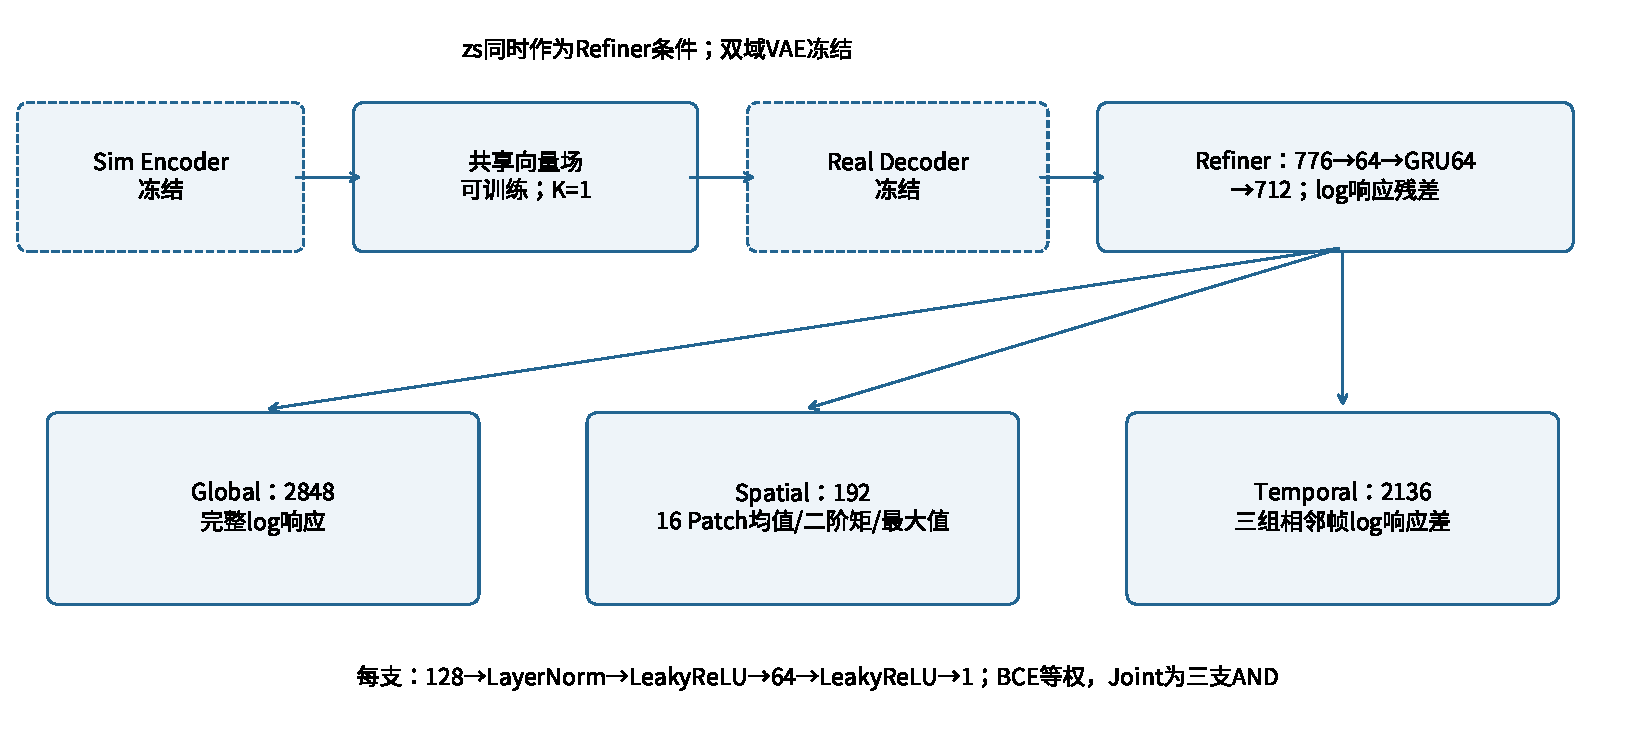
\includegraphics[width=\textwidth]{figures/ch06/multiview_refiner_architecture.pdf}
\caption{残差生成与多视角判别结构。虚线表示冻结的双域VAE；Patch仅按既定通道索引分组。}
\label{fig:ch06_multiview_refiner_architecture}
\end{figure}

图\ref{fig:ch06_multiview_refiner_architecture}中的判别输入均由归一化log响应构造，不含二值Mask。Global展平完整窗口，维数2848；Spatial汇集每帧16个Patch的均值、二阶矩和最大值，共192维；二阶矩为归一化log响应的$\operatorname{mean}(l^2)$，不是方差或标准差；Temporal使用三组相邻帧差，共2136维。这些特征分别覆盖整体响应、固定Patch内分布及短时帧差；Spatial不建立通道间物理邻接关系，Temporal差分也不是经过时间标定的物理导数。各支均为Linear至128维、LayerNorm、LeakyReLU、Linear至64维、LeakyReLU及单logit输出。三支BCE等权组合，Joint要求三支同时接受，辅助连续分数取最小logit。$D_{50}$共688643个参数，与前述判别器容量及输入均不同；未做删支后独立重训，不能归因各分支贡献或宣称同容量优势。

D训练10个Epoch、660步后冻结，G训练20个Epoch、1280步，固定取第20轮终点。采样采用全窗打乱、短域循环及全局组权重损失，并非每批严格组均衡。图\ref{fig:ch06_multiview_gradient_training}展示各Epoch首步的分支梯度诊断：三支均有有限非零梯度，能够传至共享场和Refiner，说明这些判别特征均能参与生成器更新。该诊断逐Epoch选取首批求导，描述的是这一采样范围内的梯度传递。D在生成阶段固定，VAE参数保持冻结，梯度仍可穿过Real Decoder回传；结构可导与统计约束充分是不同问题。

\begin{figure}[htbp]
\centering
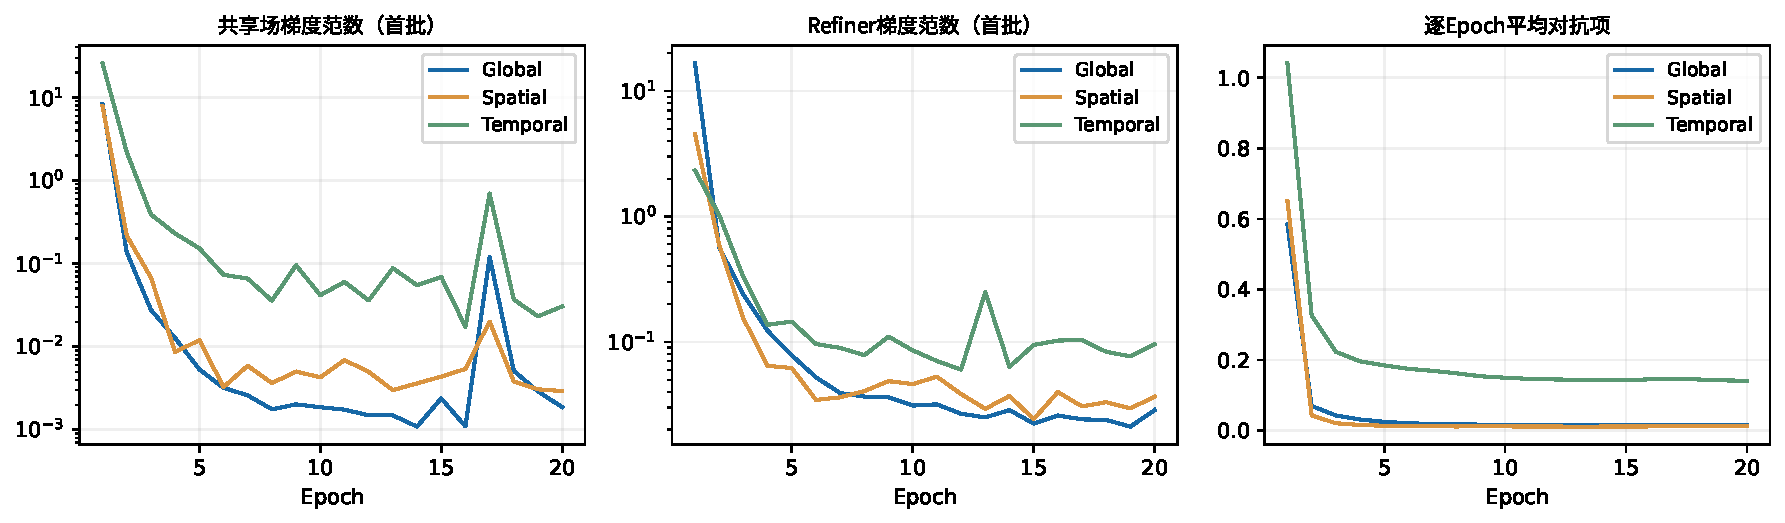
\includegraphics[width=\textwidth]{figures/ch06/multiview_gradient_training.pdf}
\caption{生成阶段各Epoch首步的分支梯度范数及逐Epoch平均对抗项。曲线来自历史训练日志，梯度非零不代表质量改善。}
\label{fig:ch06_multiview_gradient_training}
\end{figure}

\begin{table}[htbp]
\centering
\caption{固定分布评价下的生成结果与终点诊断}
\label{tab:ch06_multiview_results}
\begingroup\setlength{\tabcolsep}{4pt}
\begin{tabular}{lrrl}
\toprule
状态 & SWD & MMD & 实验角色\\
\midrule
$F_0$ & 0.206609 & 0.343678 & 初始参照\\
$F_{50}$ & 4.247227 & 0.882140 & 主结果\\
$F_{50}$终点关闭Refiner（诊断） & 0.340365 & 0.365503 & 终点诊断\\
\bottomrule
\end{tabular}
\endgroup
\end{table}

表\ref{tab:ch06_multiview_results}中终点距离明显恶化，虽然Joint FR为100\%，Real Joint接受率仅68.0833\%；两者仍分别按Root和Session宏平均。距离使用共同的冻结预处理和评价合同，避免针对终点重新调整尺度。关闭Refiner没有重训或重新选模，不能替代主结果。历史机制审计还发现，将初始输出统一放大2倍，前64个Train输出的指定检查中preserve变化为0；flow仅约束基础场修正项，不直接约束新增残差。这一检查提示：优化可以在保持相对响应关系的同时放大整体幅值，因而现有保持项仍留下幅值变化的自由度。该机制与终点退化相容，具体贡献还需受控实验区分。

数值后端也限制归因。历史初始CUDA与CPU参照最大差为1.5591305494308472，Mask相差169项；终点CUDA重载最大差约$8.58307\times10^{-6}$，满足既有allclose检查，仍有5695个近零Mask条目不同，对应响应不超过$4.76837\times10^{-7}$。未加权存储零比例约0.491242，组等权质量汇总约0.500657，二者口径不同。这些历史审计说明，相同评价规则下仍需保留推理后端及近零响应的数值差异；讨论架构效果时应将其与结构变化一并考虑。

这项单Seed探索呈现出明确的分歧：多视角约束能够影响生成器，生成样本也更易被接受，但固定距离反而退化。下一节据此从分布、邻域覆盖与输入依赖三个角度检查生成结果，以区分对判别器的适应和触觉重建质量。
